\chapter{Improving the Model}\label{chap:model_improvements}

In this chapter, I address various questions raised by the literature and use the insights from Chapter~\ref{chap:crnn} to improve the \emph{CRNN}. I perform a series of experiments to test improvements to the model, evaluate a selection of models on the test set and perform qualitative analysis of the model's outputs.

Many of these experiments introduce new hyperparameters. I choose these hyperparameters in a greedy fashion and keep them as specified unless stated otherwise. While the assumption of independence between hyperparameters is certainly be wrong, it is computationally infeasible to perform a full hyperparameter search. Selection based on greedy search is the best option available.

\section{Revisiting the Spectrogram}\label{sec:spectrogram-results}

\subsection{Spectrogram Variants}\label{sec:spectrogram-variants}

It is standard practice in ACR to use a CQT as input. However, \citet{20YearsofACR} raise the question of whether the CQT is truly the best choice. They suggest that the pitch-folding of the CQT may distort the harmonic structure of notes. By contrast, \citet{MelodyTranscriptionViaGenerativePreTraining} use a mel-spectrogram in place of a CQT. 

I test four spectrogram variants in Table~\ref{tab:spectrograms}. These include the standard CQT, mel-spectrogram and linear spectrogram. I also calculate a chroma-CQT to test whether the model is using information from multiple octaves better than a hand-crafted algorithm. The chroma-CQT is calculated by summing CQT values across octaves. Spectrogram calculations are all implemented in \texttt{librosa}~\citep{librosa}. I use $216$ bins for the CQT and mel spectrograms and $2048$ fast Fourier transform (FFT) bins for the linear spectrogram with a hop length of $4096$ for all. 

Results show that CQTs are the best choice. This raises questions as to the validity of the conclusions drawn by \citet{MelodyTranscriptionViaGenerativePreTraining}. They claim that their generative features are better than hand-crafted features. However, they only compare to mel-spectrograms which may not perform as well as CQTs for the related task of melody recognition. The CQT is also better the chroma-CQT. We can be confident that the model is using information from multiple octaves more efficiently than the simply summing across octaves.

\begin{table}[h]
    \centering
    \begin{tabular}{lccccc}
        \toprule
        spectrogram & acc & root & third & seventh & mirex \\  
        \midrule
        CQT & \textbf{60.2} & \textbf{78.4} & \textbf{75.3} & \textbf{62.5} & \textbf{79.5} \\
        chroma-CQT & 50.1 & 71.4 & 65.7 & 52.0 & 69.8 \\
        mel & 52.7 & 69.1 & 66.3 & 54.6 & 70.6 \\
        linear & 51.2 & 66.1 & 63.0 & 53.1 & 73.8 \\
        \bottomrule
    \end{tabular}
    \caption{Results for CQT, chroma-CQT, mel and linear spectrograms. The CQT is certainly the best feature. The other all perform similarly on accuracy and \text{mirex}, but the chroma-CQT does comparatively at identifying thirds and sevenths. }\label{tab:spectrograms}
\end{table}

\subsection{Hop Lengths}\label{sec:hop-lengths}

Different hop lengths have been used to calculate the CQT ranging from 512~\cite{ACRLargeVocab1} up to 4096~\citep{StructuredTraining}. In previous experiments I have used a hop length of $4096$ as is used by the authors of \emph{CRNN}~\citep{StructuredTraining}. Shorter frames would reduce the number of transition frames but require more computational cost. If frame lengths are too short, the Fourier transform may not be able to capture the harmonic structure of the audio.

In Table~\ref{tab:hop_lengths}, I test the effect of different hop lengths on the model's performance. I use a CQT with $216$ bins and a hop length of $512$, $1024$, $2048$, $4096$, $8192$ and $16384$. Results indicate that performance is similar for hop lengths of $4096$ and below. Performance suffers for greater hop lengths. While it could be argued that $2048$ does better than $4096$, this difference is small enough that it is not worth the increased computational cost. Models trained with a hop size of $2048$ take at least twice as long to train and evaluate as those trained on a hop size of $4096$.

\begin{table}[h]
    \centering
    \begin{tabular}{lccccc}
        \toprule
        hop length & acc & root & third & seventh & mirex \\  
        \midrule
        512 & 60.1 & 78.3 & \textbf{75.5} & 62.4 & \textbf{80.0} \\
        1024 & 60.2 & \textbf{78.7} & 75.2 & 62.5 & 79.6 \\
        2048 & \textbf{60.3} & 78.5 & 75.2 & \textbf{62.6} & 79.6 \\
        4096 & 60.0 & 78.1 & 75.0 & 62.2 & 79.2 \\
        8192 & 57.9 & 76.2 & 72.9 & 60.1 & 79.3 \\
        16384 & 53.3 & 71.7 & 68.0 & 55.4 & 77.9 \\
        \bottomrule
    \end{tabular}
    \caption{Results over different hop lengths for CQT calculation. Any hop length in the range $512$ to $4096$ has similar performance. For frames that are any longer, performance suffers. This is likely caused by the requirement for the model to assign a single chord class to each frame. The longer the frame, the greater potential there is for multiple chords to be playing during the frame. }\label{tab:hop_lengths}
\end{table}


\section{Decoding}\label{sec:decoding}

As observed in~\ref{sec:smoothness}, \emph{CRNN} predicts $168$ transitions per song as opposed to the $104$ seen in the ground truth data. I implement a decoding step over the frame-wise probability vectors to smooth predicted labels. Common choices for decoding models include a conditional random field (CRF)~\citep{ACRLargeVocab1, BTC} and a hidden Markov model (HMM)~\citep{BalanceRandomForestACR}. 

I first implement a HMM. The HMM treats the frame-wise probabilities as emission probabilities and the chord labels as hidden states. \citet{CQTvsChroma} note that using a transition matrix with homogeneous off-diagonal entries in the transition matrix performs similarly to using a learned transition matrix. I adopt such a transition matrix for this HMM, with a parameter $\beta$ denoting the probability of self-transition and all other transition probabilities equal to $\frac{1-\beta}{C-1}$. Decoding then follows the Viterbi algorithm~\citep{Viterbi} over the summed forward and backward pass.

A plot of the effect of $\beta$ on the model's performance and the number of transitions per song is shown in Figure~\ref{fig:hmm_beta_search}. From this plot we conclude that smoothing has little affect on the performance of the model while successfully reducing the number of transitions per song to that of the true labels. I choose $\beta = 0.15$ for the remainder of experiments as it results in $102$ transitions per song while maintaining high performance. 

\begin{figure}[H]
    \centering
    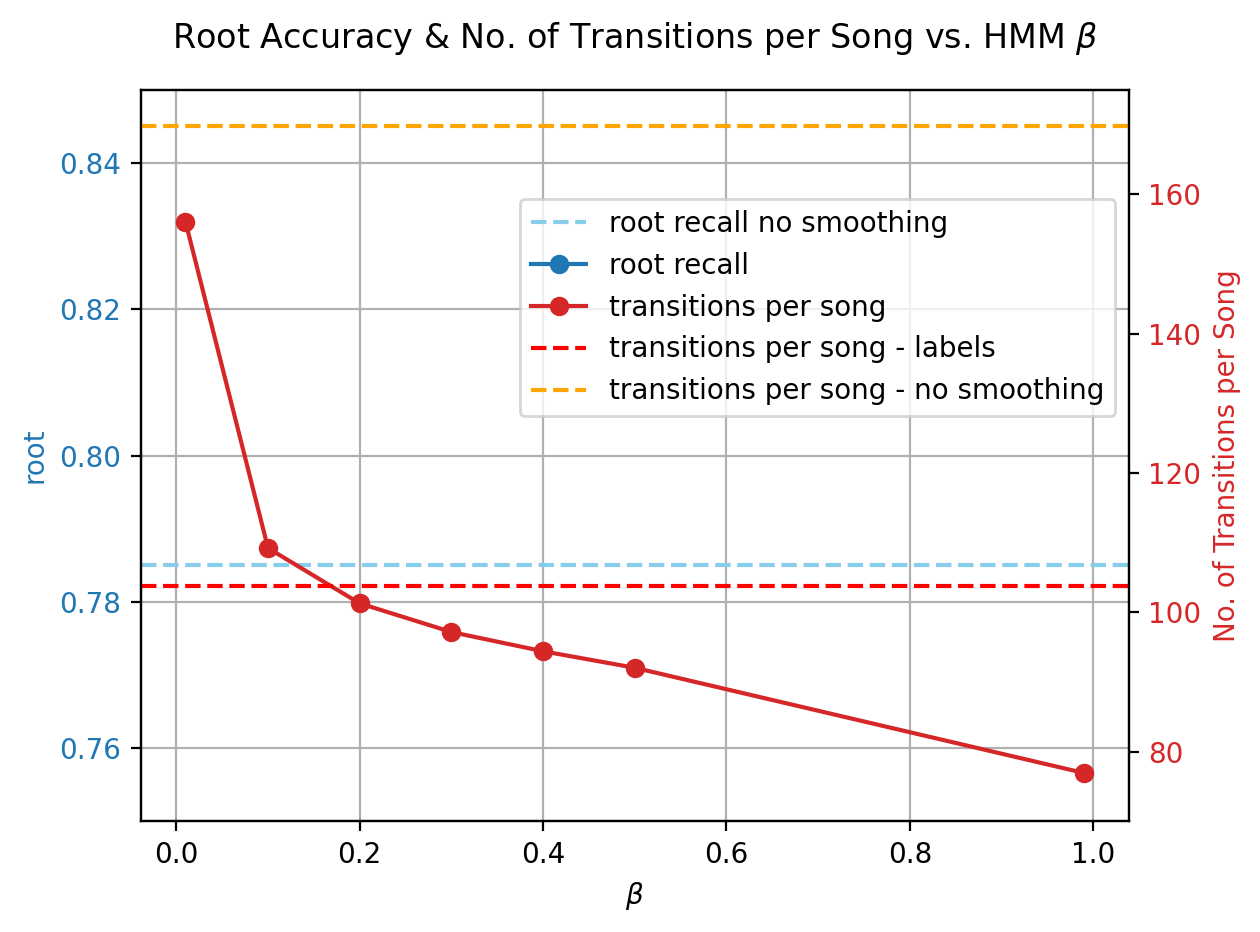
\includegraphics[width=0.8\textwidth]{figures/hmm_beta_vs_root_transitions.png}
    \caption{Effect of the HMM smoothing parameter $\beta$ on the \emph{CRNN} model. As we increase $\beta$, the number of transitions per song decreases. I choose $\beta = 0.15$ as it results in $102$ transitions per song, very close to the $104$ of the ground truth. Performance is stable across $\beta$ with a slight degradation for $\beta > 0.3$. Other performance metrics showed similarly stable results. }\label{fig:hmm_beta_search}
\end{figure}

The effect of the HMM on the incorrect regions previously discussed in Section~\ref{sec:smoothness} can be found in Appendix~\ref{app:histogram_over_region_lengths}. The HMM reduced the percentage of incorrect regions which are a single frame long from $26.7\%$ to $16.7\%$. A more intuitive way to see the effect of the HMM is to look at a section of a song which was the model previously predicted many chord transitions for. This is illustrated in Appendix~\ref{app:hmm_smoothing_effect}.

I also implement a CRF using the \texttt{pytorch-crf} package.\footnote{\url{https://github.com/kmkurn/pytorch-crf}} The CRF is a linear chain CRF with a learned transition matrix.

Results comparing the HMM, CRF and no smoothing can be found in Table~\ref{tab:smoothers}. Both the CRF and HMM reduce the number of transitions per song to a similar level. The HMM outperforms the CRF, with $3.5\%$ greater accuracy. The HMM has almost identical performance to the model with no smoothing. I hypothesise that the learned transition matrix allows the model to overfit to the chord sequences in the training set. Regardless of the explanation, I proceed with HMM smoothing.

\begin{table}[h]
    \centering
    \begin{tabular}{lcccccc}
        \toprule
        smoother & acc & root & third & seventh & mirex & transitions/song\\  
        \midrule
        none & \textbf{60.0} & \textbf{78.1} & \textbf{75.0} & \textbf{62.3} & \textbf{79.2} & 167 \\
        HMM & \textbf{60.0} &\textbf{78.1} & \textbf{75.0} & \textbf{62.3} & \textbf{79.2} & \textbf{102} \\
        CRF & 56.5 & 75.5 & 72.5 & 58.6 & 76.2 & 100 \\
        \bottomrule
    \end{tabular}
    \caption{Results for the HMM and CRF smoothing methods on \emph{CRNN}. The HMM has almost identical performance to the model with no smoothing. However, it drastically reduces the number of transition per song to an acceptable level. The CRF performs notably worse than the HMM. }\label{tab:smoothers}
\end{table}

\section{The Loss Function}

\subsection{Weighted Loss}\label{sec:weighted_loss}

One of the biggest problems with \emph{CRNN} is the low recall on rarer chord qualities. Two common methods for dealing with long-tailed distributions are weighting the loss function and over-sampling. \citet{CurriculumLearning} also explore the use of curriculum learning as form of re-sampling which we do not explore here because they report only minor performance gains. Sampling is explored by \citet{BalanceRandomForestACR} but they use a different model based on pre-computing chroma vectors and re-sampling these chroma vectors for use in training a random forest for frame-wise decoding. 

In our setting, re-sampling training patches of audio may be interesting to explore but is left as future work. It would require a complex sampling scheme as frames cannot be sampled independently. 

Weighting has been explored by \citet{ACRLargeVocab1}. We employ a similar but simpler implementation here. A standard method of weighting is to multiply the loss function by the inverse of frequency of each, with a parameter controlling the strength of the weighting. This is defined in Equation~\ref{eq:weighting}.

\begin{equation}\label{eq:weighting}
    w_c = \frac{1}{{(\text{count}(c) + 10)}^\alpha}
\end{equation}

Where $w_c$ is the weight for chord $c$, $\text{count}(i)$ is the number of frames with chord $c$ in the dataset and $\alpha$ is a hyperparameter controlling the strength of weighting. $\alpha=0$ results in no weighting and increasing $alpha$ increases the severity of weighting. We add $10$ in the denominator to avoid dividing by $0$ and to diminish the dominating effect of chords with very few occurrences. I then define normalised weights $w_c^*$ in Equation~\ref{eq:weighted_loss} so that the learning rate can remain the same.

\begin{equation}\label{eq:weighted_loss}
    w_c^* = \frac{w_c}{s} \text{ where } s = \frac{\sum_{c\in \mathcal{C}} \text{count}(c)\cdot w_c}{\sum_{c\in \mathcal{C}} \text{count}(c)}
\end{equation}

Where $\mathcal{C}$ is the set of all chords in the vocabulary. This keeps the expected weight over samples at $1$ such that the effective learning rate remains the same. These values are calculated over the training set. I test values of $\alpha$ in the set \{0, 0.05, 0.1, \ldots, 0.95, 1\}. The plot in Figure~\ref{fig:weighted_loss} illustrates the effect of the weighting on the model's performance.

\begin{figure}[H]
    \centering
    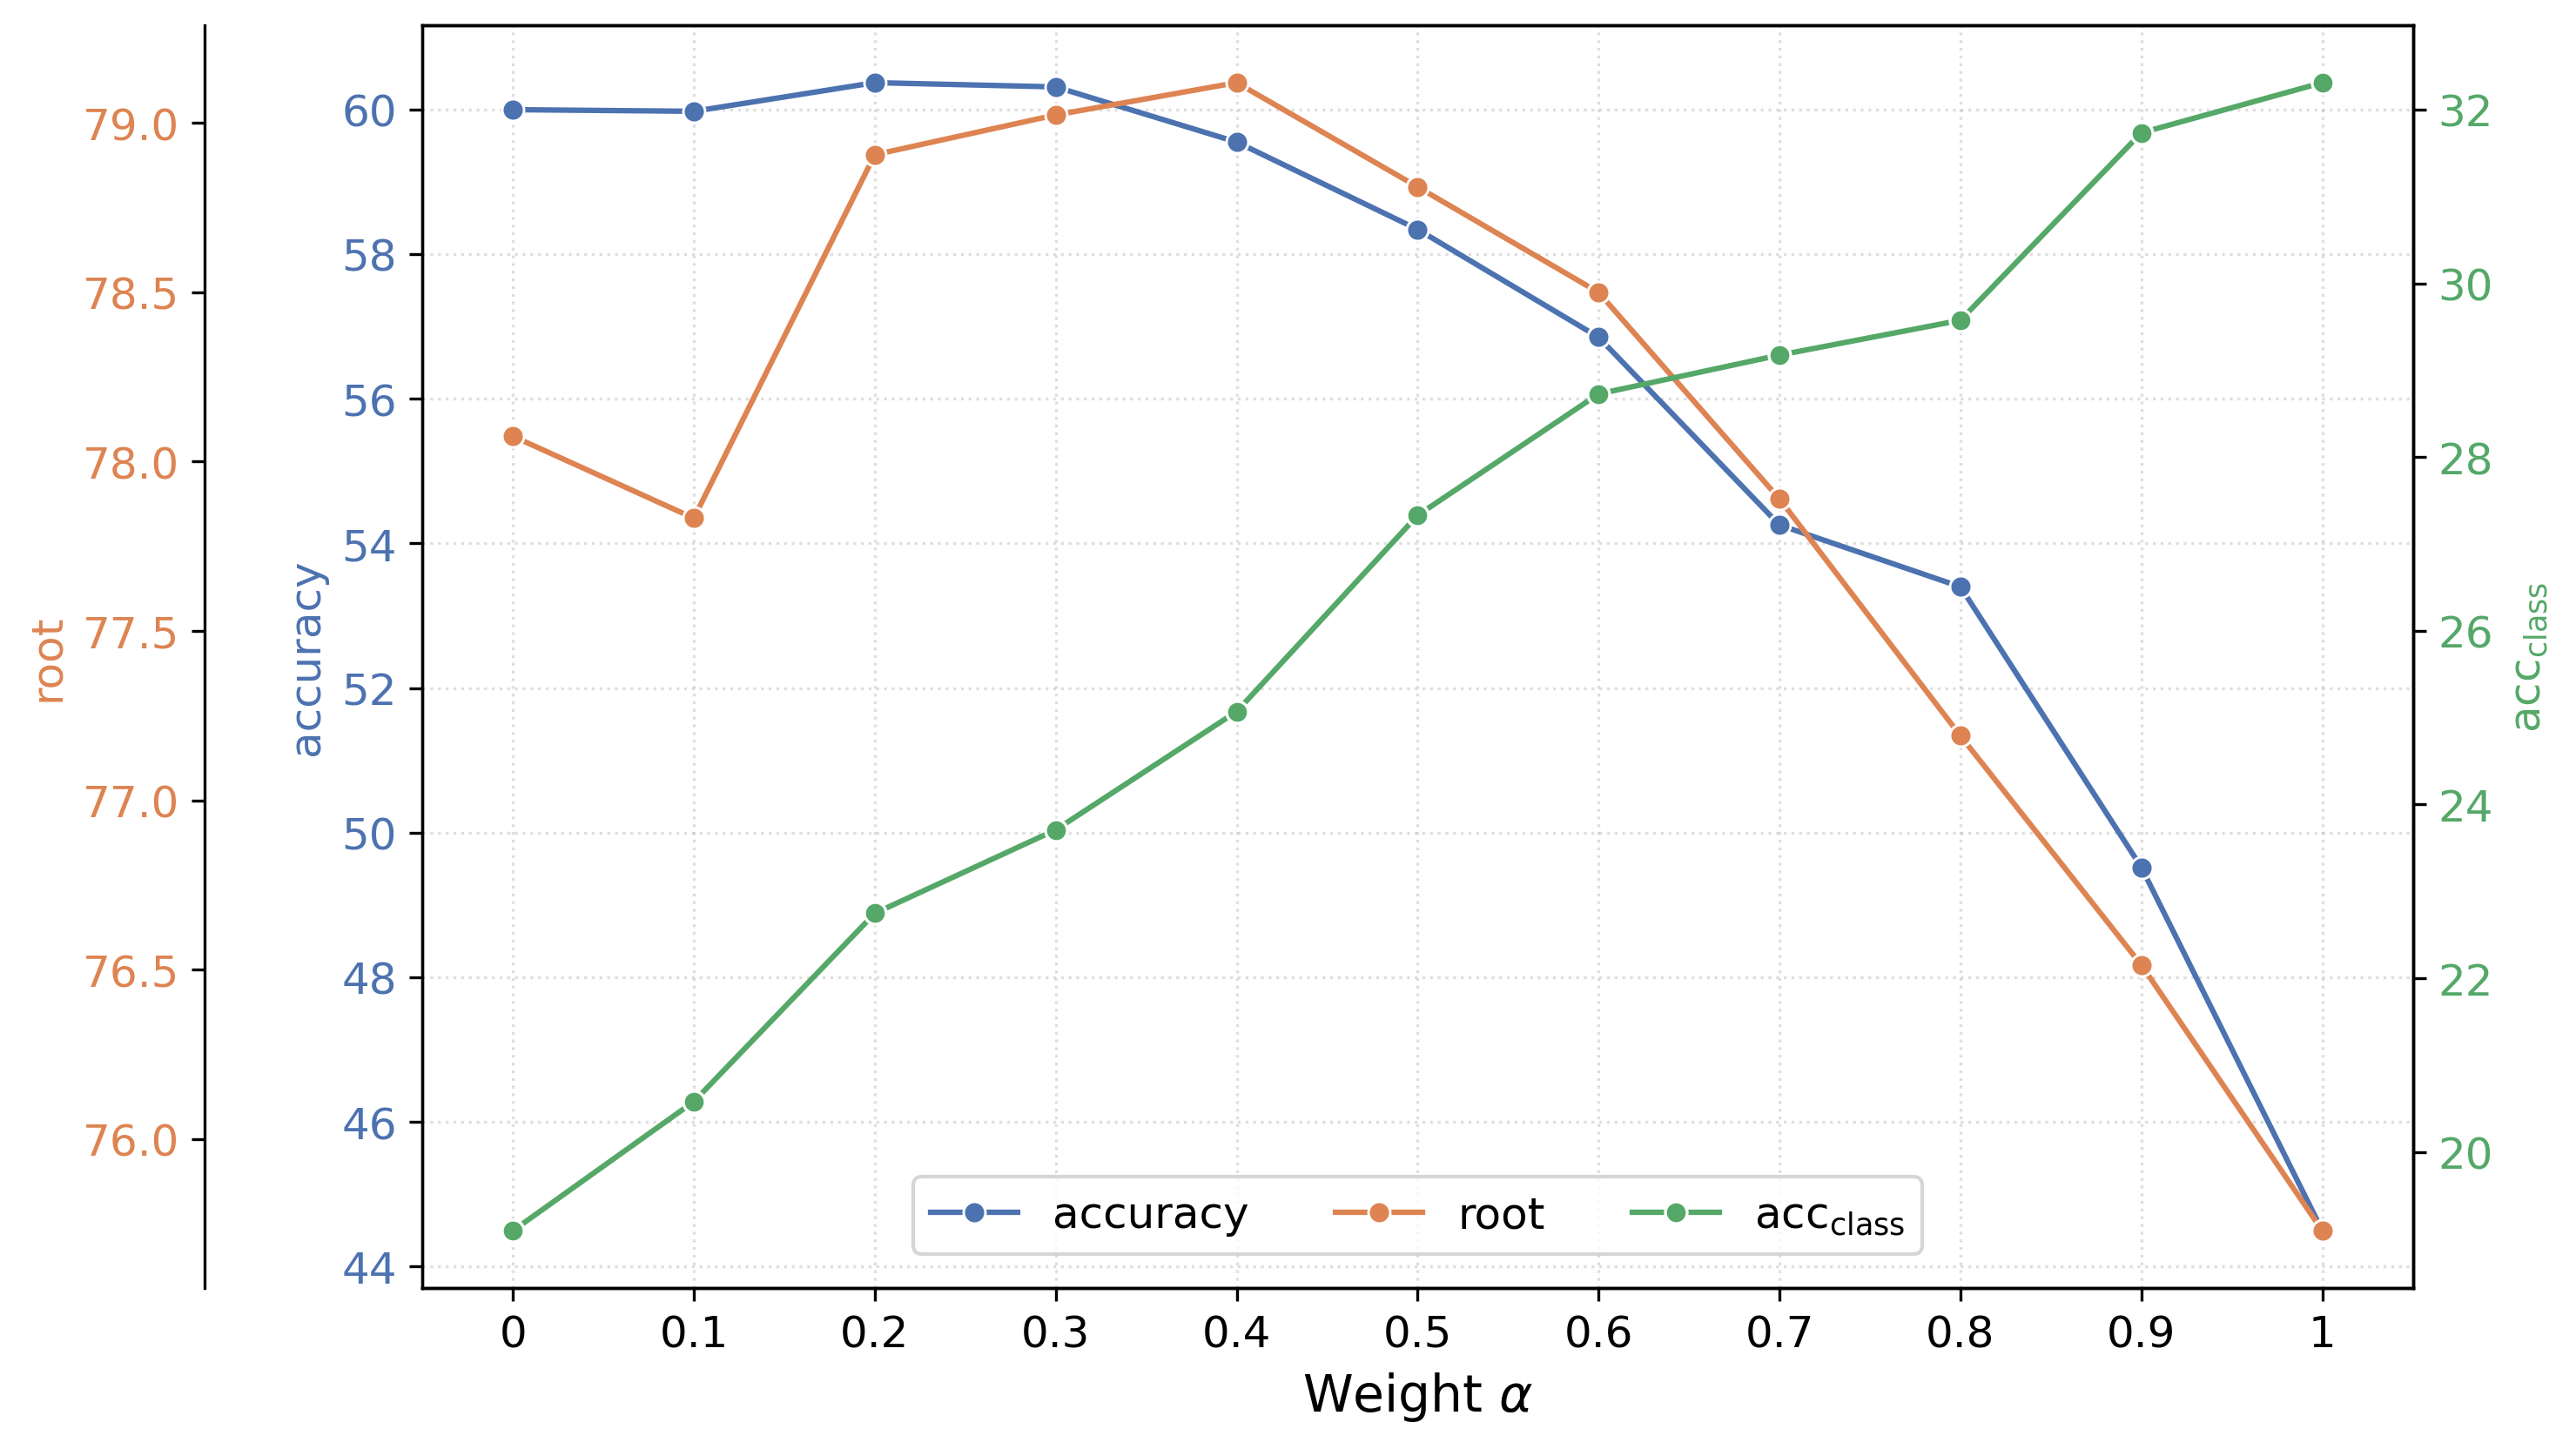
\includegraphics[width=1.0\textwidth]{figures/weight_alpha_search_trim.png}
    \caption{Effect of weighted loss on the \emph{CRNN} model with varying $\alpha$. As we increase $\alpha$, \texttt{acc}\textsubscript{class} improves accuracy and \texttt{root} decrease. I claim there is a sweet-spot where very little overall performance is sacrificed for better class-wise accuracies. I choose this to be $\alpha = 0.3$. The \texttt{root} and \texttt{third} metrics improve and less than $3\%$ is lost on other metrics while mean class-wise accuracy improves by $6\%$ and the median improved by $0.2$. This plot also reveals strong correlation between metrics. }\label{fig:weighted_loss}
\end{figure}

For further insight, a plot of the differences between a confusion matrices with and without weighted loss can be found in Appendix~\ref{app:weighted_loss_confusion_matrix}. Notably, recall on most qualities increases, with recall on major7 doubling to $0.34$. The weighted model predicts $2.2$ times fewer \texttt{X} symbols which may explain how it increases recall on these rarer qualities without sacrificing on accuracy. 

Weighting the loss function also increased the number of transitions predicted per song slightly. This may be because occasional sharp gradient updates cause more extreme probability outputs. I increase the HMM smoothing parameter $\beta$ to $0.2$ to bring the number of transition per song to $104$.

\subsection{Structured Loss}\label{sec:structured_loss}

\citet{StructuredTraining} propose a structured loss function which they claim improves performance on the \emph{CRNN} model. They introduced additional targets of the root, bass and pitch classes. I follow a similar method but do not include the bass as the current chord vocabulary does not consider inversions. The idea behind this loss term is to explicitly task the model with identifying the components of a chord that we care about. This can allow the model to exploit structure in the chord vocabulary such as shared roots and pitch classes, rather than all symbols being predicted independently.

The root can be any of the 12 notes in the Western chromatic scale, \texttt{N} or \texttt{X}, creating a 14-dimensional classification problem. The 12 pitch classes each represent a single binary classification problem. Two fully connected layers calculate a 14-dimensional vector and 12-dimensional vector from the hidden representation outputted from the GRU for the root and pitch classes respectively. Finally, these representations are concatenated with the original output of the model and fed to the final fully connected layer to predict the chord symbol.

The mean cross-entropy loss is calculated in each case. These are then summed to from the \emph{structured loss}. Finally, a linear combination of the structured loss and the original loss is calculated. The final loss is a convex combination of the original loss and the structured loss as defined in Equation~\ref{eq:structured_loss}.

\begin{equation}\label{eq:structured_loss}
    L = \gamma L_{chord} + (1-\gamma)(L_{root} + L_{pitch})
\end{equation}

Where $L$ is the overall loss, $L_{chord}$ is the cross-entropy loss over chords symbols, $L_{root}$ is the cross-entropy loss targeting the root, $L_{pitch}$ is mean binary cross-entropy over each of the pitch classes. $\gamma$ is a hyperparameter controlling the weighting of the original loss. 

The plot in Figure~\ref{fig:structured_loss} illustrates the effect of the structured loss on the model's performance. Choosing $\gamma=0.7$ improves accuracy by $1.3\%$ while \texttt{mirex} worsens by $0.3\%$. Accuracy with \texttt{third} increases by $1.7\%$ and on \texttt{seventh} by $1.3\%$. I keep $\gamma=0.7$ going forward.

\begin{figure}[H]
    \centering
    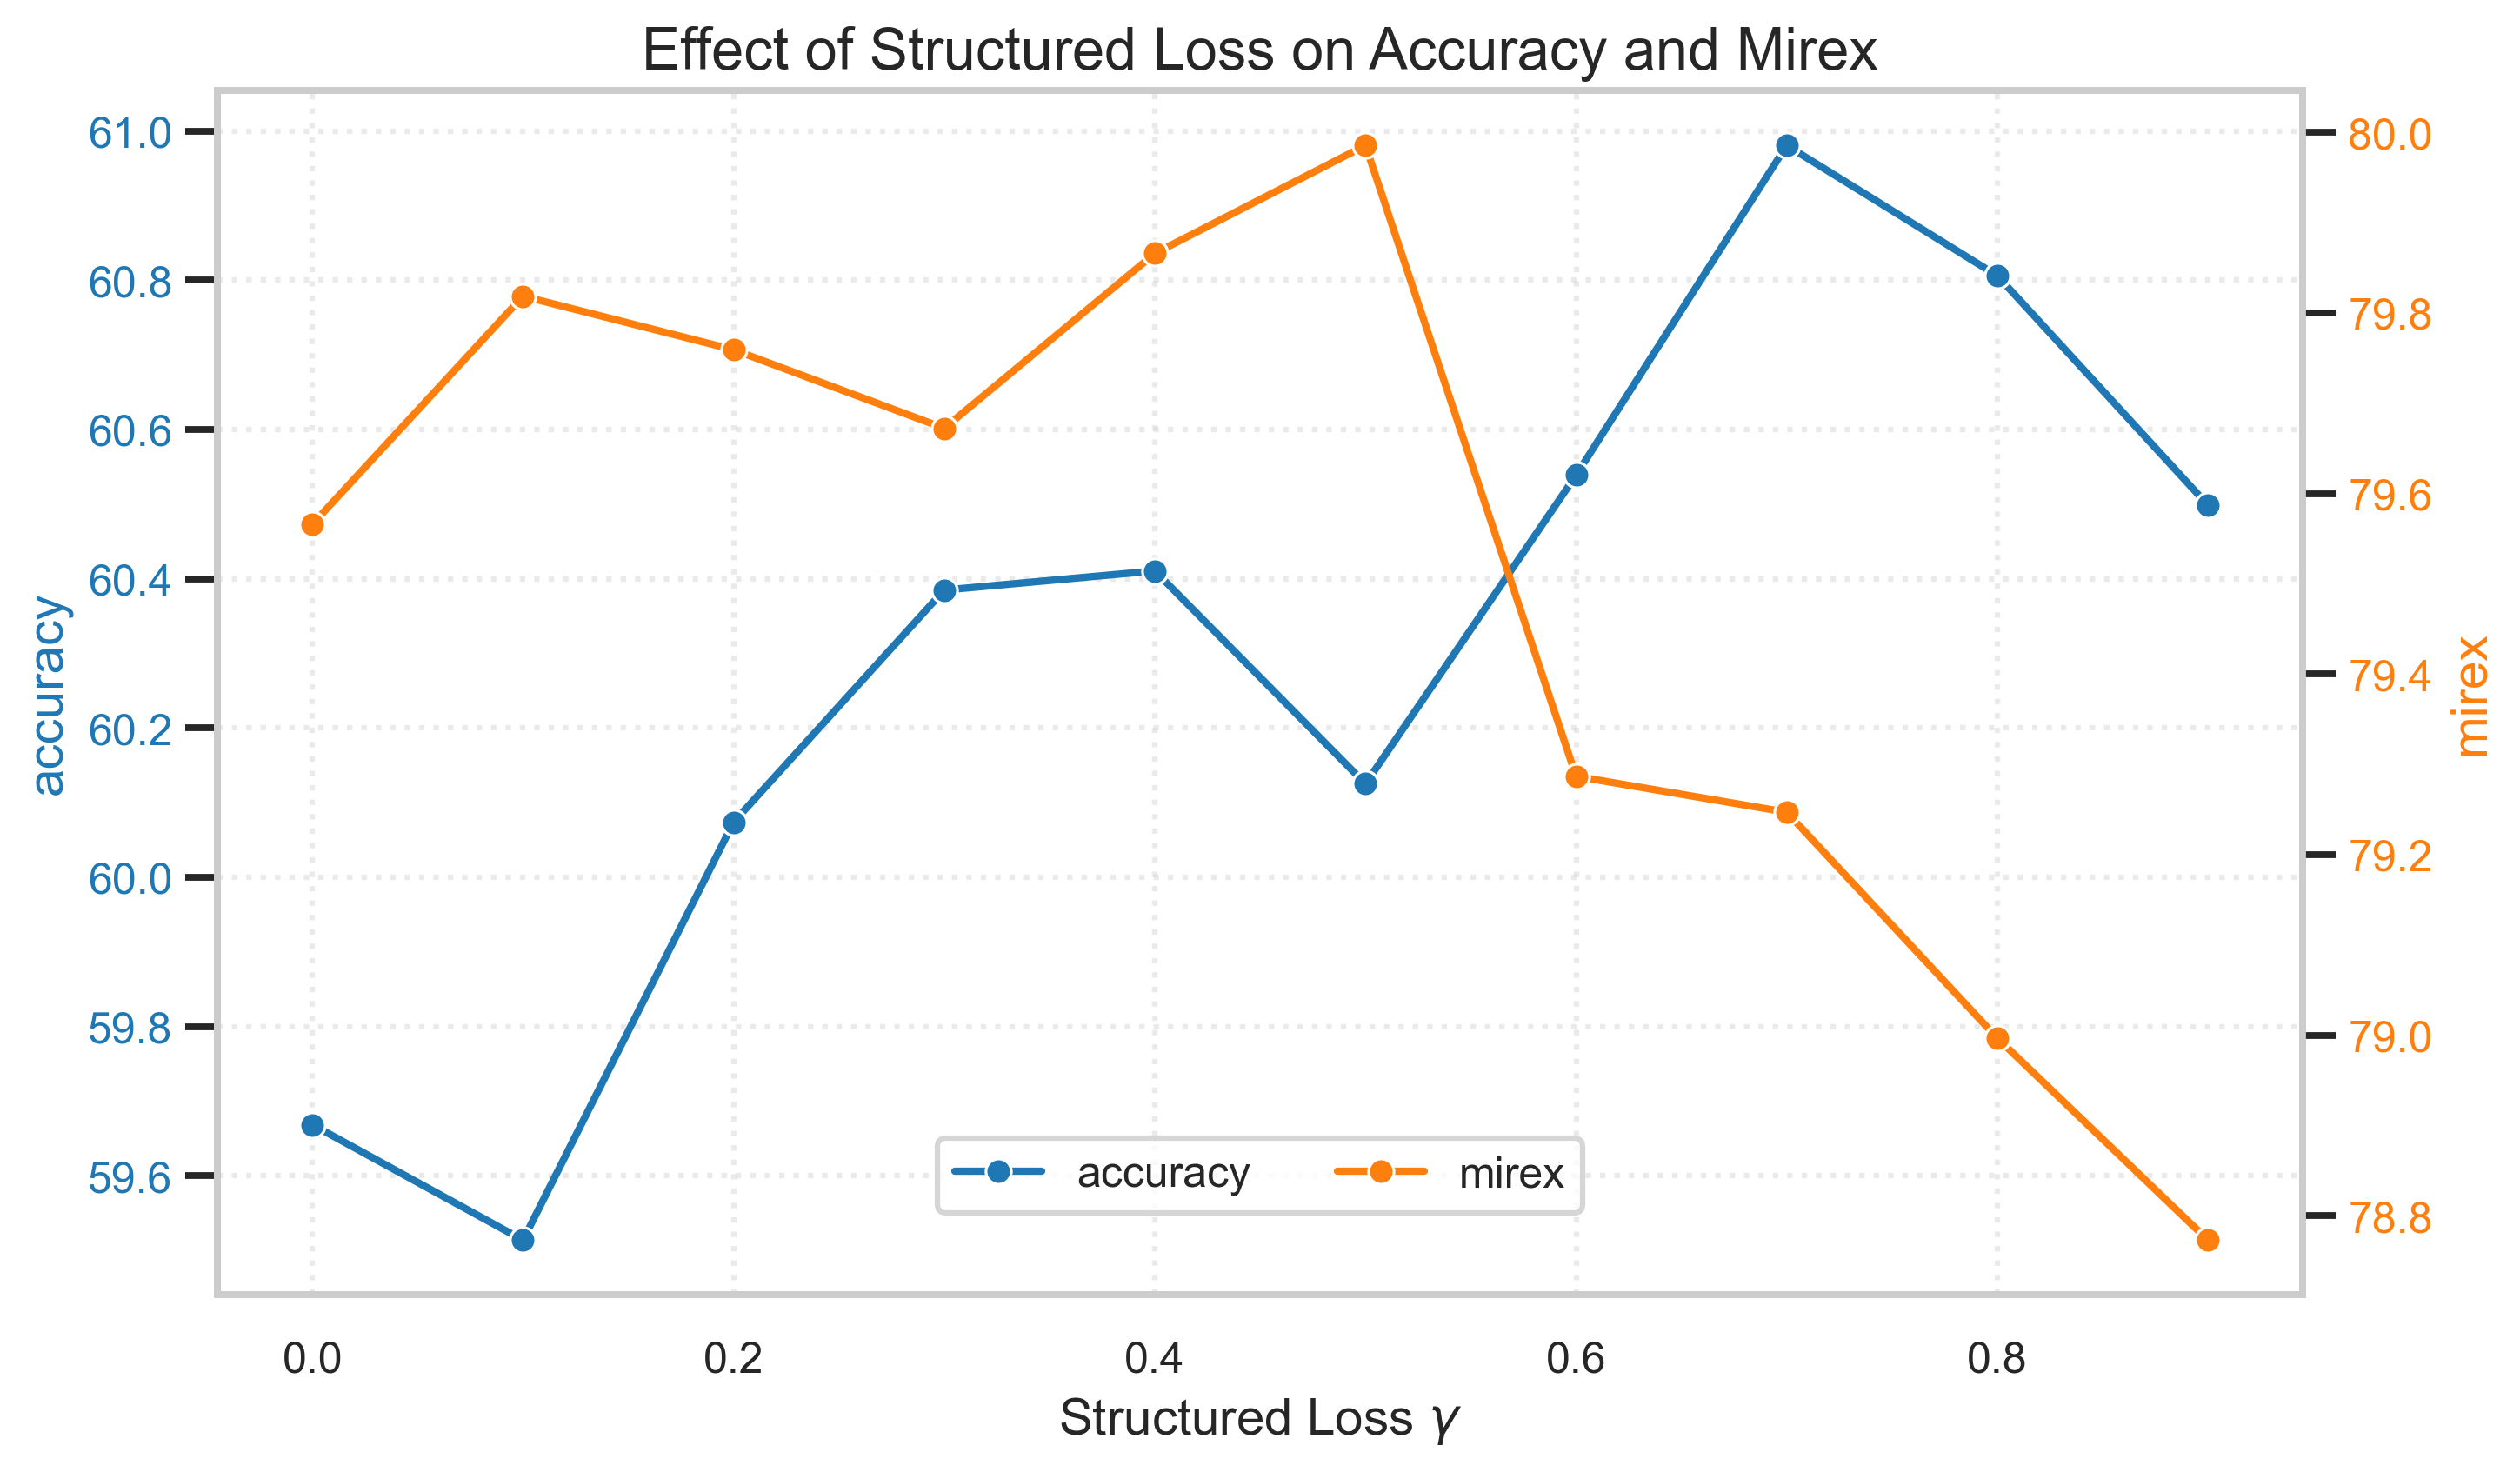
\includegraphics[width=1.0\textwidth]{figures/structured_loss_accuracy.png}
    \caption{Effect of structured loss on the \emph{CRNN} model with varying $\gamma$. As we increase $\gamma$, accuracy improves but \texttt{mirex} behaves erratically, worsening at the higher end. The other metrics behave similarly to accuracy. I choose $\gamma=0.7$ based on peak accuracy. }\label{fig:structured_loss}
\end{figure}

\section{Generative Features}

\citet{MelodyTranscriptionViaGenerativePreTraining} use generative features extracted from Jukebox~\citep{Jukebox} to improve performance for melody transcription. They also produce a chord transcription model using the same methodology but do not report results. I decide to test generative features using MusicGen~\citep{MusicGen} as a feature extractor. This was for several reasons. MusicGen is a newer model. It has several different sizes of model which could be tested against each other as an experiment on the complexity of the model. It has a fine-tuned variant called MusiConGen~\citep{MusiConGen} which is used for synthetic data generation in Section~\ref{sec:synthetic_data}. All model weights are available on the HuggingFace Hub.\footnote{\url{https://huggingface.co/docs/hub/en/index}} Finally, its training data was properly licensed, unlike Jukebox. I leave the results of Jukebox for future work.

\textbf{Feature Extraction}: Overlapping $5$ second chunks of audio were fed through MusicGen in a batched fashion. This first requires passing the audio through the pre-trained Encodec audio tokeniser~\citep{Encodec}. These are then fed through the language model. I take the output logits as the representation for each frame. The model outputs logits in four `codebooks', each $2048$-dimensional vectors, intended to represent different granularities of detail in the audio. Audio segments are overlapped such that every frame has context from both directions. The multiple representations for each frame are averaged. Finally, these representations are upsampled. The model operates at a frame rate of 50Hz. To compute a representation with the same frame length as the CQT, I take the mean over the frames outputted by the model closest to the centre of the CQT frame. In case averaging over frames dampened the signal, I also tried linearly interpolating between the two closest frames outputted by the model. However, this was empirically found to perform slightly worse. Results are left to Appendix~\ref{app:linear_interpolation_vs_area_averaging}. This feature extraction required the use of NVIDIA RTX A6000 GPUs. The extraction process takes 4 hours for each model over the entire dataset.

As the representations are $2048$-dimensional, it is computationally infeasible to feed this directly into the GRU. Instead, I project these vectors down into a smaller dimensionality. I tested learned fully connected layers which reduce down to dimension of powers of $2$, from $16$ to $1024$. The best representation was found to be with a projection down to $64$ dimensions, although the results showed no clear trend. Results are left to Appendix~\ref{app:projection_dimensionality}.

I test the use of different variants of MusicGen and reductions of the four codebook representations. I test musicgen-large (3.3B parameters), musicgen-small (330M), musicgen-melody (1.5B) and MusiConGen (1.5B). I train models on each codebook separately, on the element-wise mean across codebooks or the concatenation of all four. The best model was found to be musicgen-large and the best reduction to average over the four codebooks. However, results were all close. They are left to Appendices \ref{app:generative_feature_extraction_models} and \ref{app:generative_feature_extraction_reductions} for lack of interest.

It might be argued that it is better to use musicgen-small to save on computational cost but the dimensionality of the codebooks is the same across all model variants. Once the features have been extracted, they are all equally as expensive to train on.

It is surprising that the concatenated representation performs worse than the averaged representation as it contains at least as much information. However, if the information provided by each of the codebooks is largely the same then there are no reasons that the concatenated representation should perform better and training may simply find a worse minima. Regardless, training on $8192$-dimensional vectors is computationally very expensive, even with dimensionality reduction.

To test whether or not these features help when compared with a CQT, I test with the CQT only, generative features only and a concatenation of the two. The results are shown in Table~\ref{tab:gen_feature_comparison}. Although the generative features perform worse than the CQT, they clearly contain information useful for chord recognition with an accuracy of $58.7\%$. When the CQT and generative features are used together, performance remains largely the same. This experiment was run multiple times, with similar results each time. There is no clear evidence that the generative features provide any benefit over just using the CQT. 

This is surprising as \citet{MelodyTranscriptionViaGenerativePreTraining} claim that generative features are better than hand-crafted features for the related task of melody recognition. However, they only compare to mel-spectrograms which do not perform as well as CQTs. Conclusions here cast doubt on the validity of their claims. It may be the case that features extracted from other generative models such as Jukebox~\citep{Jukebox} or MusicLM~\citep{MusicLM} may perform better. The comparison is left for future work.

Given the lack of improvement and the drastically increased computational cost associated with extracting features and training the model, I do not proceed with using generative features.

\begin{table}
    \centering
    \begin{tabular}{lccccc}
        \toprule
        features & accuracy & root  & third & seventh & mirex \\  
        \midrule
        gen$\cdot$CQT  & \textbf{61.0}     & \textbf{80.3}  & \textbf{77.0}  & \textbf{63.3}    & 78.4  \\
        gen      & 58.7     & 77.6  & 74.3  & 60.9    & 77.5  \\
        CQT      & \textbf{61.0}     & 79.8  & 76.8  & 63.2    & \textbf{79.3}  \\
        \bottomrule
    \end{tabular}
    \caption{Comparison of CQT and generative features with a concatenation of the two, denoted as gen$\cdot$CQT. The concatenation performs the best on most metrics, but not by enough to claim that it is meaningfully better. }\label{tab:gen_feature_comparison}
\end{table}

\section{Pitch Augmentation}\label{sec:pitch-augmentation}

Pitch augmentation has been done in other works on chord recognition, either on the CQT~\citep{ACRLargeVocab1} by shifting the CQT bins up or down or directly on the audio~\citep{BTC,StructuredTraining}. Although similar, these are not identical transformations. Shifting the CQT takes place after discarding phase information and leaves empty bins behind whereas audio pitch shifting can introduce other artefacts intended to preserve harmonic structure and maintain phase information. I implement both methods and compare.

When a sample is drawn from the training set, it is shifted with probability $p$. The shift is measured in semitones in the set $\{-5,-4\ldots -1, 1, \ldots 6\}$ with equal probability of each shift. This means there is 12 times as much training data. Convergence was still reached in 150 epochs. Shifting the CQT matrix is done by moving all items up or down by the numbers of bins corresponding to the number of semitones in the shift. The bins left behind after the shift are filled with a value of -80dB. Audio shifting is done with \texttt{pyrubberband}.\footnote{\url{https://github.com/bmcfee/pyrubberband}}. CQTs are calculated on the shifted audio. A plot of the effect of the shift probability $p$ on the model's performance can be found in Figure~\ref{fig:pitch_augmentation}.

Results show a clear trend that increasing $p$ improves performance. Shifting the audio provides a very similar effect to simply shifting the CQT. Choosing $p=0.9$ results in a $2.1\%$ increase in accuracy, and an increase of $1-2\%$. The \texttt{mirex} score breaks the trend with performance varying over different values for $p$. \texttt{acc}\textsubscript{class} also improves by over $2\%$. This can be explained by the model being forced to become root-invariant. With $p=0.9$, all notes in the Western chromatic scale become almost equally likely. I proceed with pitching shifting with $p=0.9$ on the CQT for the remainder of the experiments, as it is computationally cheaper than shifting the audio.

\citet{StructuredTraining} claim an increase of $5\%$ on the median across most metrics. I do not find such a large effect here. Nonetheless, it is clear that pitch shifting is a useful augmentation.

Note that the weights for the weighted loss are calculated based on \emph{expected} counts, taking the shift probability $p$ into account. I also tested shifting with both methods at once but results were not any different than shifting with either method alone. Unfortunately, it was not computationally feasible to test pitch shifting with generative features as the feature extraction over $12 * 1210 = 14,520$ songs is too expensive.

\begin{figure}[H]
    \centering
    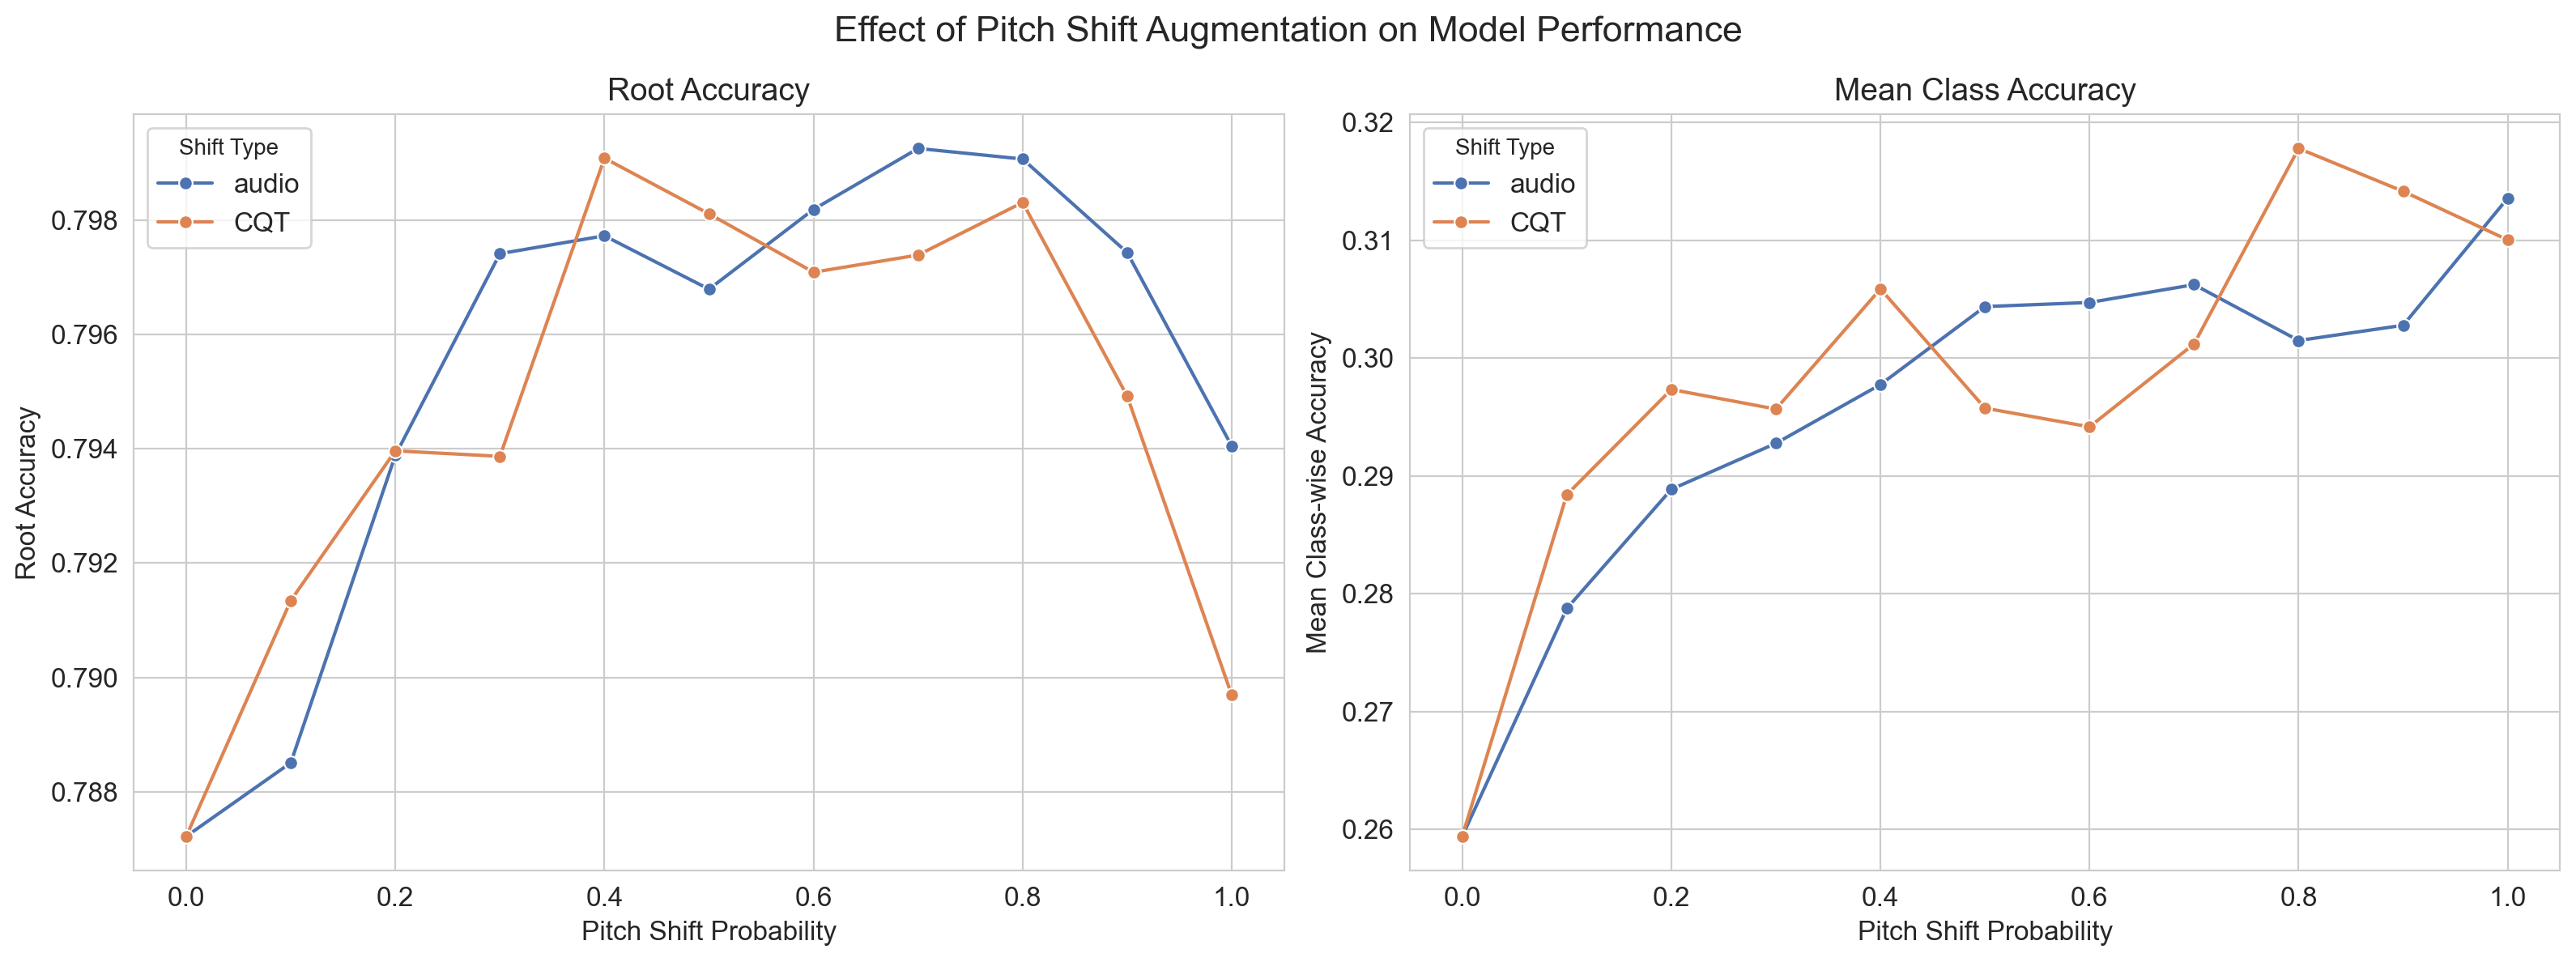
\includegraphics[width=0.8\textwidth]{figures/pitch_shift_analysis.png}
    \caption{Effect of pitch augmentation on the \emph{CRNN} model with varying $p$. Pitch shifting provides a clear increase in performance. Shifting the audio or the CQT has a similar effect. I choose $p=0.9$ which is close to making the model root-invariant.}\label{fig:pitch_augmentation}
\end{figure}


\section{Synthetic Data Generation}\label{sec:synthetic_data}

Given the success of pitch augmentation for ACR, it is sensible to look for other sources of data. Other methods of augmentation are possible such as adding noise and time-stretching. However, these do not provide new harmonic structure beyond pitch shifting or create new instances of rare chords, so I do not explore these here.

Instead, I look to generate new data. This has not been possible until recently with the advent of chord-conditioned generative models like MusiConGen~\citep{MusiConGen} and CocoMulla~\citep{CocoMulla}. I choose to use MusiConGen as it is a more recent model and the authors claim that it adheres more closely to chord conditions. Indeed they feed the outputted audio through BTC~\citep{BTC} and find \texttt{triads} score of $71\%$ using the chord conditions as ground truth. While far from perfect, it suggests the model is able to generate audio that mostly lines up with the chord conditions.

I generate $1210$ songs, each $30$ seconds long, to mimic the size of the \emph{pop} dataset. I refer to this dataset as \emph{synth}. This is split into a training, validation and testing set in the same fashion as for the \emph{pop} dataset. To generate a larger order of magnitude of songs would require a lot of compute. While the model does support auto-regressive generation for longer audio, I found that its outputs became incoherent using the provided generation functions. It also sometimes produced incoherent output with $30$ seconds, but this was much less common.

To generate a song, I sample a BPM from a normal distribution with mean $117$ and standard deviation $27$, clipped to lie in the range $[60,220]$. These values were calculated from the training set. I then sample a song description from a set of $20$ description generated by ChatGPT. The descriptions outline a genre, mood and instrumentation. Descriptions include only genres jazz, funk, pop and rock which were all part of the fine-tuning training set for MusiConGen. Note that the model does not output melodic vocals, owing to the lack of vocal music in the pre-training and fine-tuning data. Finally, I generate a jazz chord progression using the theory of functional harmony~\citet{GenerativeGrammarJazz}. Details of this process can be found in Appendix~\ref{app:jazz_chord_progression_generation}. The process generates a very different chord distribution, with many more instances of upper extensions and rare qualities. This is intended to provide the model with many more instances of rare chords. 

To offset this new distribution shift in the training data, I calibrate the probabilities outputted by the model. To encourage root-invariance, these calibration terms are averaged over roots for each quality. This calibration process is detailed in Appendix~\ref{app:calibration}, with a figure showing the calibration terms for each quality. This figure shows that the rarer qualities are much more common in the synthetic data.

Outputs from MusiConGen were manually inspected. In general, the outputs are good. They consistently stick to the provided BPM and normally stick to the chord conditions. The outputs could be musically unpleasant, especially with less realistic chord transitions and some of the rarer chord qualities. They also did not have a huge variety in terms of timbre and instrumentation. Nonetheless, they provide examples of audio that could be annotated in a sensible manner by a human.

I compare a model trained on only \emph{pop}, trained on only synthetic data, and trained on both. While the latter results in more training data per epoch, convergence is always reached so these are fair comparisons. I test the models on both the \emph{pop} and synthetic data test sets. The results are shown in Table~\ref{tab:synthetic_data}. Given the increased instances of rare chords in the synthetic data, I remove the weighting on the loss function for the models trained on synthetic data.

\begin{table}[h]
    \centering
    \begin{tabular}{lcc}
        \toprule
        training set & \emph{pop} acc & \emph{synth} acc \\  
        \midrule
        \emph{pop} & \textbf{62.1} & 24.2 \\
        \emph{synth} & 48.6 & 44.8 \\
        both & \textbf{62.1} & \textbf{51.0} \\
        \bottomrule
    \end{tabular}
    \caption{Results for models trained on the Pop dataset, synthetic data and both together. Unsurprisingly models trained on \emph{pop} perform better on \emph{pop} and models trained on \emph{synth} perform better on \emph{synth}. The model trained on both does not to any better on the \emph{pop} validation split, but performance is increased on the \emph{synth} validation split. Training only on \emph{pop} results in an accuracy of just $24.2\%$ on \emph{synth}, much lower than reported by \citet{MusiConGen}. However, this may be due to the unrealistic distribution of chords in the generated sequences. }\label{tab:synthetic_data}
\end{table}

The model trained on both datasets performs very similarly to the model only trained on \emph{pop} on the \emph{pop} validation split. That is, the model has not overfitted to the synthetic data and become worse at recognising the \emph{pop} dataset. However, it has also not improved performance. Training on any synthetic data drastically improves the accuracy on the \emph{synth} validation split. This is likely due to the unique chord distribution of the generated jazz progressions and the consistent but unrealistic instrumentation. The model trained on both datasets performs the best, with an accuracy of $51.0\%$.

For further insight, the difference in confusion matrix over qualities is plotted in Appendix~\ref{app:cm_synthetic_data}. It does not show any clear trends. Recall on some rare qualities increases while it decreases for others. In general, the model predicts \texttt{maj} less often for rare chord qualities but replaces this with more varies erroneous predictions.

While performance does not improve, the lack of overfitting and the improvement on the synthetic data provides hope that with further work, different chord progressions and improved generative models, synthetic data generation could prove a useful tool for ACR. Given the lack of performance increase, I do not continue to train on the synthetic data for remaining experiments.

\section{Beat Synchronisation}\label{sec:beat-synchronisation}

Chords exist in time. Musicians interpret chords in songs as lasting for a certain number of beats, not a fixed length of time. In its current form, the model outputs frame-wise predictions. While these could be stitched together to produce a predicted chord progression or beat-wise predictions could be made as a post-processing step, I decide to implement a model that outputs beat-wise predictions directly. This allows the model to use information from the entire duration of the beat to make its prediction.

Following the methodology of \citet{MelodyTranscriptionViaGenerativePreTraining} for melody transcription, I first detect beats for every song in the dataset using \texttt{madmom}~\citep{madmom}. This returns a list of time steps where beats have been detected. While this model is comparable to state-of-the-art, I first verify that the beats are plausible. I performed a cross-correlation analysis with the chord transitions in a similar manner to Section~\ref{sec:data-integrity}. A histogram of maximum lags within a window of $0.3$ seconds can be found in Appendix~\ref{app:beat_histogram}. I find that almost all maximum lags occur within a window of $0.1$ seconds, while the minimum beat length is $0.27$ seconds and mean is $0.52$ seconds. In order to provide more evidence, I compute the maximum accuracy a model could attain if predicting chords at the beat level. This is done by iterating over each beat interval and assigning the chord with maximum overlap with the ground truth. This yields an accuracy of $97.1\%$. With these observations combined, I am satisfied that beat-wise predictions will not limit the model.

\citet{MelodyTranscriptionViaGenerativePreTraining} task the model will producing predictions for every 1/16th of a beat. However, such fast transitions are not necessary for chord recognition. The possible accuracy of $97.1\%$ over beats suggests that the model need only predict once every beat interval.

To calculate features for a beat interval, I average all CQT features whose centre is contained within the beat. The CQT is calculated using a hop length of $1024$. The shorter hop length was used to minimise the effect of CQT frames with partial overlap with two beat intervals. This also ensures that each beat has many CQT frames associated with it, even when using fractions of a beat interval. As noted in Section~\ref{sec:hop-lengths}, this does not impact performance. Increased computational cost is not a concern as beat-wise representations have a much lower frequency than a CQT with frame length of $4096$.

I test the model with different divisions and groupings of beats. This is to test the assumption that the whole beats are fine-grained enough for the model to make good predictions. I include tests where beat intervals are sub-divided in two, in four, or beat intervals are joined into groups of two and four. I refer to this as the \emph{beat division}. I also test a \emph{perfect} beat division where the true chord transitions are taken as the beats. This is not a fair comparison as the model should not have access to the chord transition timings. However, it does provide an idea of how the model would fare if the beat intervals were `perfect' in the sense that $100\%$ accuracy is possible. Note that HMM smoothing is removed for beat-wise models as the model is now predicting at the beat level.

Results are shown in Table~\ref{tab:beat_division}. Forcing the model to produce beat-wise predictions does not affect performance compared to frame-wise predictions with a hop length of $4096$. The model also performs just as well with a beat division of $1$ as with a beat division of $1/2$ or $1/4$, suggesting that the beats produced by \texttt{madmom} are already at the correct level of granularity. The model performs meaningfully worse with a beat division of $2$ or $4$. 

The model with `perfect' beat intervals performs slightly worse on accuracy metrics but attains a very high \texttt{mirex} score of $90.4\%$ which is the highest of any seen in the literature. This is a new result which provides sorely needed hope for significant improvements in the field. If a model is able to achieve $90.4\%$ \texttt{mirex} score, then it may be possible for accuracy metrics to be brought up to a similar level. This is a very promising result. Why the model performs worse on accuracy metrics is not clear. It may be because averaged features from longer time periods provide better information as to the pitch classes present but dampens signal regarding the root note. Indeed, the mean chord duration is $1.68$ seconds while a CQT frame is $0.093$ seconds. Why this effect is not observed when predicting at the beat-level is also not clear. Further analysis is required to understand this. Such analysis may lead to insights that allow significant improvements in the field.

\begin{table}[H]
    \centering
    \begin{tabular}{lccccc}
        \toprule
        beat division & acc & root & third & seventh & mirex \\  
        \midrule
        1/4                 & 62.3           & 81.3          & 78.3          & 64.5           & 79.6         \\
        1/2                 & \textbf{62.8}  & 81.5          & \textbf{78.6} & \textbf{65.1}  & 79.9         \\
        1                   & 62.3           & 81.3          & 78.1          & 64.6           & 80.0         \\
        2  & 56.4           & 74.7          & 71.6          & 58.5           & 73.4         \\
        4 & 50.8           & 68.0          & 64.5          & 52.8           & 67.2         \\
        none                & 62.5           & \textbf{81.7} & 78.2          & 64.7           & 80.2         \\
        perfect             & 61.1           & 79.6          & 76.1          & 63.4           & \textbf{90.4}\\
        \bottomrule
    \end{tabular}
    \caption{Results for different beat divisions. The beat division of `none' refers to a frame-wise \emph{CRNN} with a hop length of $4096$ and HMM smoothing applied and `perfect' refers to intervals that are calculated from the labels. Note that this `perfect' model is not a fair test. Beat-wise predictions with beat intervals of $1$ and below see no decrease in performance compared to frame-wise predictions. Beat intervals greater than $1$ increasingly suffer from being forced to assign predictions to larger periods of time that may not line up with true chord transitions. Interestingly, a beat interval of 2 still performs relatively well. A notable result is the \texttt{mirex} score of the `perfect' model. A score of $90.4\%$ is the highest of any in the literature. Despite this, its accuracy is not improved. It is not entirely clear why. }\label{tab:beat_division}
\end{table}


\section{Final Results}\label{sec:test-set}

For final results, I retrain select models on the combined training and validation splits and test on the held out test split. This is an 80/20\% train/test split. I consider the original \emph{CRNN} with no improvements, \emph{CRNN} with a weighted and structured loss and HMM smoothing, concatenating generative features with CQTs, pitch augmentation, beat-wise recognition, `perfect' beat-wise recognition and training on synthetic data. 

Results are shown in Table~\ref{tab:test_set}. The model with the best performance on the test set is the \emph{CRNN} with perfect beat tracking. Observations are largely similar to those found previously. Weighted and structured loss with smoothing improve accuracy by $1.2\%$, with pitch shifting improving by a further $1\%$. Generative features do not help but synthetic data improves performance by a further $0.6\%$. This alone is not a clear enough signal that the model is better but provides hope for further work in using synthetic data. Beat-wise resampling does not harm performance while the `perfect' model achieves the highest performance across all metrics. The \texttt{mirex} of $90\%$ has reduced to $88.7\%$, and the gap with accuracy has closed when compared with results in Table~\ref{tab:beat_division}. 

The mean class-wise accuracy does not improve past $19.7\%$ without `perfect' beats. The median in this case is $6\%$. The model's performance on the long tail remains poor. Using a greater $\alpha$ in weighting may improve the picture but would require sacrificing accuracy.

\begin{table}[H]
    \centering
    \begin{tabular}{lcccccc}
        \toprule
         & acc & root & third & seventh & mirex & acc\textsubscript{class} \\
        \midrule
        \emph{CRNN}               & 61.6  & 79.3  & 76.5  & 63.3  & 80.6  & 18.9 \\
        + weighted/structured/HMM & 62.8  & 80.9  & 78.3  & 64.6  & 80.6  & 18.6 \\
        + gen features           & 62.7  & 80.4  & 77.9  & 64.6  & \textbf{80.6}  & 19.5 \\
        + pitch shift           & 63.8  & \textbf{82.4}  & 79.4  & 65.6  & 80.3  & \textbf{19.7} \\
        + synthetic data         & \textbf{64.4}  & 82.2  & \textbf{79.9}  & \textbf{66.3}  & \textbf{81.5}  & 18.3 \\
        \midrule
        + perfect beats          & 65.8  & 84.5  & 81.7  & 67.6  & 88.7  & 21.2 \\
        \bottomrule
    \end{tabular}
    \caption{Results from various experimental setups. The `perfect beats' model assumes oracle beat tracking and achieves the highest results across all metrics but is excluded when considering the best results for each metric as it is not a fair comparison. Beat-wise models do not use synthetic data. Metrics progressively increase as we introduce various new elements. Adding the weighted loss, structured loss term and an HMM smoother improves accuracy by $1.2\%$. Generative features do not help. Pitch shifting improve by a further $1\%$, and synthetic data by a further $0.6\%$.}\label{tab:test_set}
\end{table}


\section{Qualitative Analysis}
